% если хочется, можно поставить 14pt
\documentclass[12pt, dvipsnames]{extarticle}

\usepackage{luatex85}
\pdfminorversion=5

\usepackage{fontspec}
\usepackage{polyglossia}
\usepackage[a4paper, 
lmargin=30mm, rmargin=15mm, tmargin=20mm, bmargin=20mm]{geometry}
\usepackage{multirow}

\usepackage{pgfplots}
\pgfplotsset{compat=1.18}

\setdefaultlanguage{russian}
\setotherlanguage{english}

% Согласно требованиям к ВКР
\defaultfontfeatures{Ligatures=TeX}

\setmainfont{Times New Roman}
\setmonofont{Courier New}
\setsansfont{Arial}

\newfontfamily\cyrillicfont{Times New Roman}
\newfontfamily\cyrillicfontsf{Arial}
\newfontfamily\cyrillicfonttt{Courier New}

\newfontfamily\englishfont{Times New Roman}
\newfontfamily\englishfontsf{Arial}
\newfontfamily\englishfonttt{Courier New}

\linespread{1.5}

\usepackage{titlesec}

\titleformat{\section}{\normalfont\fontsize{14}{14}\bfseries}{\thesection}{1em}{}
\titleformat{\subsection}{\normalfont\fontsize{14}{14}\bfseries}{\thesubsection}{1em}{}
\titleformat{\subsubsection}{\normalfont\fontsize{14}{14}\bfseries}{\thesubsubsection}{1em}{}

\setlength{\parindent}{1.25cm}

\renewcommand\thesection{\arabic{section}}

\usepackage[a-1b,mathxmp]{pdfx}
\hypersetup{hidelinks,colorlinks=true,citecolor=BurntOrange,urlcolor=Blue}

\usepackage[backend=biber,
bibencoding=utf8,
sorting=none,
style=gost-numeric,
language=autobib,
autolang=other,
clearlang=true,
defernumbers=true,
sortcites=true,
doi=true,
isbn=true,
]{biblatex}

\renewcommand{\UrlFont}{\small\rmfamily\tt}
\appto{\bibsetup}{\raggedright}

\bibliography{bibliography/betti}
%\bibliography{bibliography/}


\usepackage{amsfonts}

\usepackage{tikz}
\usepackage{pgfplots}
\usepackage{wrapfig}

\usepackage{caption}
\usepackage{subcaption}

\usepackage{amsfonts, amssymb, amsmath, amsthm}
\usepackage{mathtools}
\usepackage{enumerate}
\usepackage{verbatim}

\usepackage{mathrsfs,amsfonts,mathtools}
\usepackage{amsmath}          
\usepackage{amssymb}

\usepackage{amsthm} 
\usepackage{thmtools}

\usepackage{graphicx} 
\graphicspath{{images/}}

\renewcommand{\emptyset}{\varnothing}
\renewcommand{\epsilon}{\varepsilon}
\renewcommand{\phi}{\varphi}
\renewcommand{\kappa}{\varkappa}

\begin{document}
	\setcounter{page}{2}
	
	\vspace*{\fill}
	\begin{abstract}
		Согласно генетическому исследованию аутосомных маркеров и митохондриальной ДНК 979 домашних, диких и одичавших кошек с трёх континентов, в том числе барханных кошек (Felis margarita), все домашние кошки по материнской линии происходят как минимум от пяти представительниц подвида степная кошка (Felis silvestris lybica), имеющих разные гаплотипы митохондриальной ДНК. В митохондриальной гаплогруппе IV, специфической для ближневосточных и домашних кошек, идентифицировали 6 субклад и рассчитали время жизни общего предка — ок. 13 тыс. лет назад, что значительно превышает время предполагаемого одомашнивания ближневосточных кошек.
	\end{abstract}
	\vspace*{\fill}
	
	\newpage
	\tableofcontents
	\newpage
	
	% !TEX root = ../diploma.tex
\section{Физиология}
\subsection{Cубфизиология}

Частота пульса у взрослых кошек варьирует в зависимости от физической и психической активности и составляет от 120 до 220 ударов в минуту. Частота дыхания составляет в среднем 20—40 дыхательных движений в минуту.

\[x^n = \mathbb{R}^n + y^n\]

\section{Вопрос о полном одомашнивании}

В наше время среди учёных нет точного ответа, является ли кошка полностью одомашненным животным, так как, например, собака в процессе одомашнивания изменила свою модель поведения, сумев развить довольно сильную привязанность и преданность к человеку, и одновременно утратила множество способностей к охотничьему образу жизни и сигнальному общению, присущих её предкам — волкам.

\begin{figure}
	\centering
	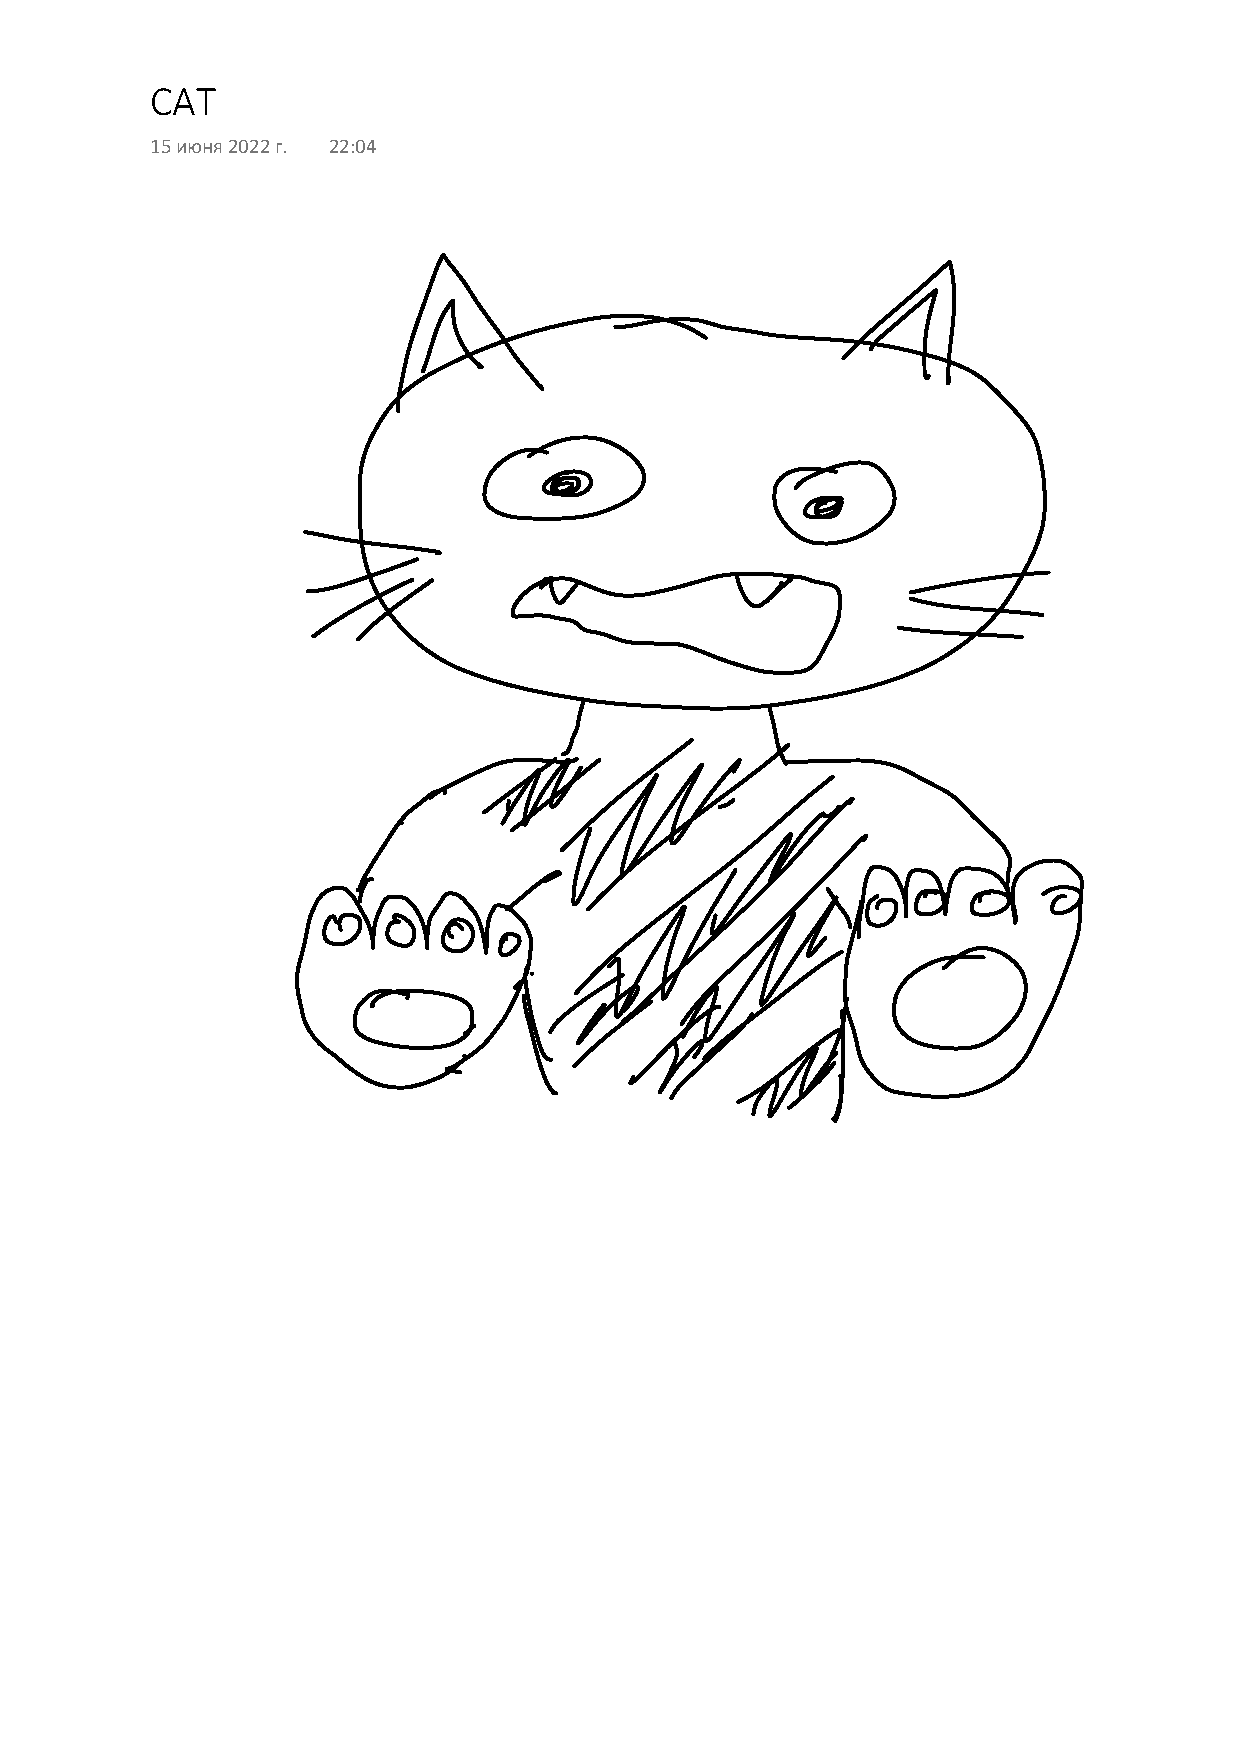
\includegraphics[clip, trim=2cm 2cm 2cm 2cm, width=0.3\textwidth]{cat}
	\caption{Название $\mathbf{Cat}$}
	\label{fig:im1}
\end{figure}

На картинке \ref{fig:im1}, смотреть в \cite{betti}.

	\newpage
	\printbibliography
\end{document}